\section{Grundlagen}

\begin{frame}{Ein typisches Freifunk Netz}
    todo Bild eines typischen Freifunk Netzes
\end{frame}

\begin{frame}{Unser grobes Ziel}
    \includegraphics[width=\textwidth]{img/svg/freifunk_konzepte.pdf}

    Unser Freifunknetz ist in mehrere Layer-2 Inseln, die per Layer-3 miteinander verbunden sind,
    aufgeteilt. Die Hoods A und B in diesem Beispiel sind über unser VPN jeweise mit einem Router im
    Internet verbunden. Hood C hat einen lokalen Router, der direkt am LAN-Port hängt.
\end{frame}

\begin{frame}{Mesh-Router}
    \begin{itemize}
        \item OpenWRT mit
        \item Batman-Adv
        \item Fastd
        \item Nodewatcher
        \item Fastdstart
        \item .. weiteren kleineren Tools
        \item .. configs und scripten
    \end{itemize}
\end{frame}

\begin{frame}{Mesh-Router von aussen}
    \begin{itemize}
        \item Client-Ports \& Infrastructure Funknetz:
            Wie ein großer Switch
        \item Batman-Ports \& Ad-Hoc Funknetz:
            Mesh-Netz
        \item WAN-Ports:
            VPN Netz
    \end{itemize}
    \center{
        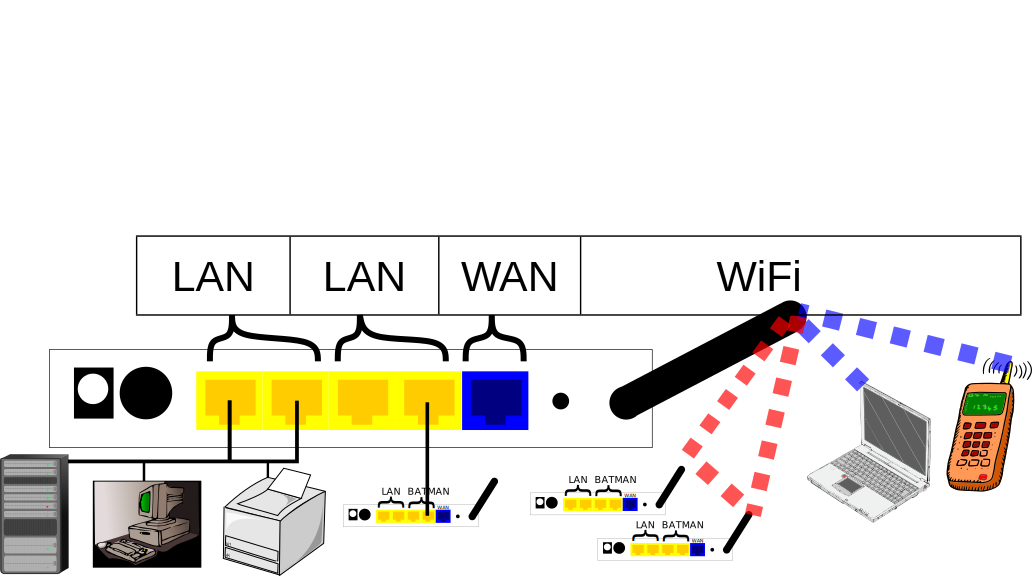
\includegraphics[width=0.75\textwidth]{img/svg/anschluesse.pdf}
    }
\end{frame}

\begin{frame}{Mesh-Router von innen}
    \renewcommand{\arraystretch}{1.5}
    \begin{tabular}{|c|c|c|c|c|c|c|} \hline
         \multicolumn{7}{|c|}{Bridge} \\ \hline
         \multirow{2}{*}{Managed} &
         \multicolumn{4}{c|}{B.A.T.M.A.N} &
         \multicolumn{2}{c|}{\multirow{2}{*}{Client-VLan}} \\ \cline{2-5}
         & Ad-Hoc & VPN & \multicolumn{2}{c|}{Node-VLan} & \multicolumn{2}{c|}{} \\ \hline
         \multicolumn{2}{|c|}{Wifi} & WAN & LAN1 & LAN2 &
         LAN3 & LAN4 \\ \hline
    \end{tabular}

    \begin{itemize}
        \item Jeder Knoten ist wie ein großer Switch
    \end{itemize}
\end{frame}

\begin{frame}{Allgemeines}
    \begin{itemize}
        \item Verwendetes VPN: fastd
        \item Layer-II Netz
        \item Wir nutzen keine Verschlüsselung (! :-O)
    \end{itemize}
    \begin{block}{fastd}
        % todo: was ist fastd ?
        There are no server and client roles defined by the
        protocol, this is just defined by the usage.
        \begin{itemize}
            \item Only one instance of the daemon is needed on each
                host to create a full mesh
            \item If no full mesh is established, a routing protocol
                is necessary to enable hosts that are not connected
                directly to reach each other
        \end{itemize}
    \end{block}
\end{frame}

\begin{frame}{Gateway}
    \begin{itemize}
        \item VPN
        \item DHCP
        \item DNS
        \item Policy base routing
        \item Routing zu anderen Gateways
        \item Optional Routing ins Internet
    \end{itemize}
\end{frame}

\begin{frame}{Monitoring}
    \begin{itemize}
        \item z.B. Netmon
        \item Was tut es? ..
    \end{itemize}
\end{frame}
